\section{Results}
\subsection{Results of the datasets}
The results of the experiment were gathered by taking a 1000 photos of the particles in the trap and for each of the laser power output ($P$) settings and then using an automated MATLAB script to track the location of the centre of the bead for all of the 1000 photos and all of the laser output power settings. Using this information the script was able to calculate the trap stiffness in the $x$ and $y$ direction denoted as $k_x$ and $k_y$ respectively.\\
The script was not perfect, for most of the image stacks of the first dataset the script was not able to track the centre of the bead, this was the result of a piece of debris in the trap which was like the bead circularly shaped with rings around it, this threw the program off. The corresponding data points have been entered in the table \ref{tab:first-results} below but the points were not used for fitting a line to the dataset. The second dataset was much better and did not have any faulty measurements, its values are shown in table \ref{tab:second-results}.\\

\vspace{-.2cm}
\begin{table}[h!]
\centering
\begin{tabular}{|l|l|l|l|l|l|l|}
\hline
Laser Power {[}$mW${]} & 0*         & 10*        & 20        & 30*        & 40         & 40        \\ \hline
$k_x$    {[}$pN/nm${]}        & $2.36 \cdot 10^{-5}$ &$ 2.45 \cdot 10^{-7}$ & $1.60\cdot 10^{-5}$  & $8.35\cdot 10^{-7}$ & $1.99\cdot 10^{-5}$  & $9.60\cdot 10^{-5}$ \\ \hline
$k_y$     {[}$pN/nm${]}       & $8.29 \cdot 10^{-5}$ &$ 2.94\cdot 10^{-7}$ & $1.65\cdot 10^{-5}$ & $9.71\cdot 10^{-7}$ & $1.72\cdot 10^{-5}$ & $8.96\cdot 10^{-5}$ \\ \hline
\end{tabular}
\caption{Results of the first dataset. The values are truncated to two decimal places. * denotes a faulty measurement}
\label{tab:first-results}
\end{table}


\vspace{-.2cm}
\begin{table}[h!]
\centering
    \begin{tabular}{|l|l|l|l|l|l|l|}
        \hline
        Laser Power {[}$mW${]} & 0         & 5         & 10         & 20         & 30         & 40         \\ \hline
        $k_x$     {[}$pN/nm${]}       & $3.64\cdot 10^{-7}$ & $8.24\cdot 10^{-5}$ & $1.08\cdot 10^{-4}$ & $3.03\cdot 10^{-4}$ & $6.14\cdot 10^{-4}$ & $7.55\cdot 10^{-4}$ \\ \hline
        $k_y$     {[}$pN/nm${]}       & $5.55\cdot 10^{-7}$   & $4.18\cdot 10^{-5}$ & $2.53\cdot 10^{-5}$  & $1.10\cdot 10^{-4}$ & $1.69\cdot 10^{-4}$ & $2.54\cdot 10^{-4}$ \\ \hline
    \end{tabular}
\caption{Trap results, values are truncated to two decimal places for formatting reasons}
\label{tab:second-results}
\end{table}

\vspace{-.5cm}
\begin{minipage}{\linewidth}
    \centering
    \begin{minipage}[l]{0.45\linewidth}
        \begin{figure}[H]
            \centering
            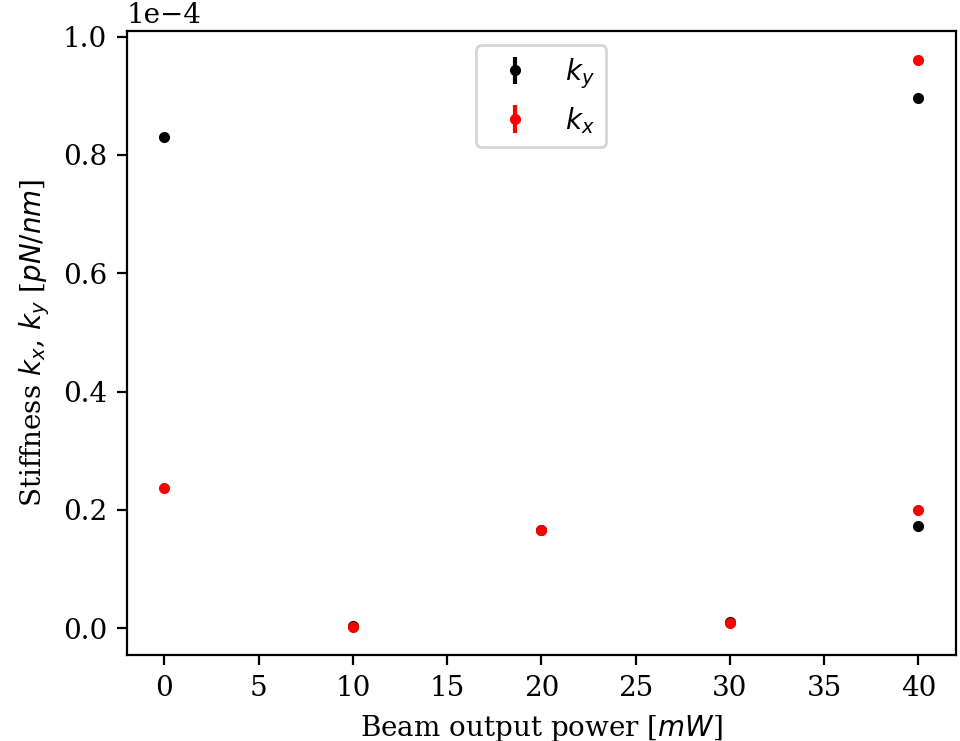
\includegraphics[width=\linewidth]{figures/beam.png}
            \caption{Results of the first dataset plotted and fitted.\\}
            \label{fig:bead-plot}
        \end{figure}
    \end{minipage}
    \hspace{0.05\linewidth}
    \begin{minipage}[r]{0.45\linewidth}
        \begin{figure}[H]
            \centering
            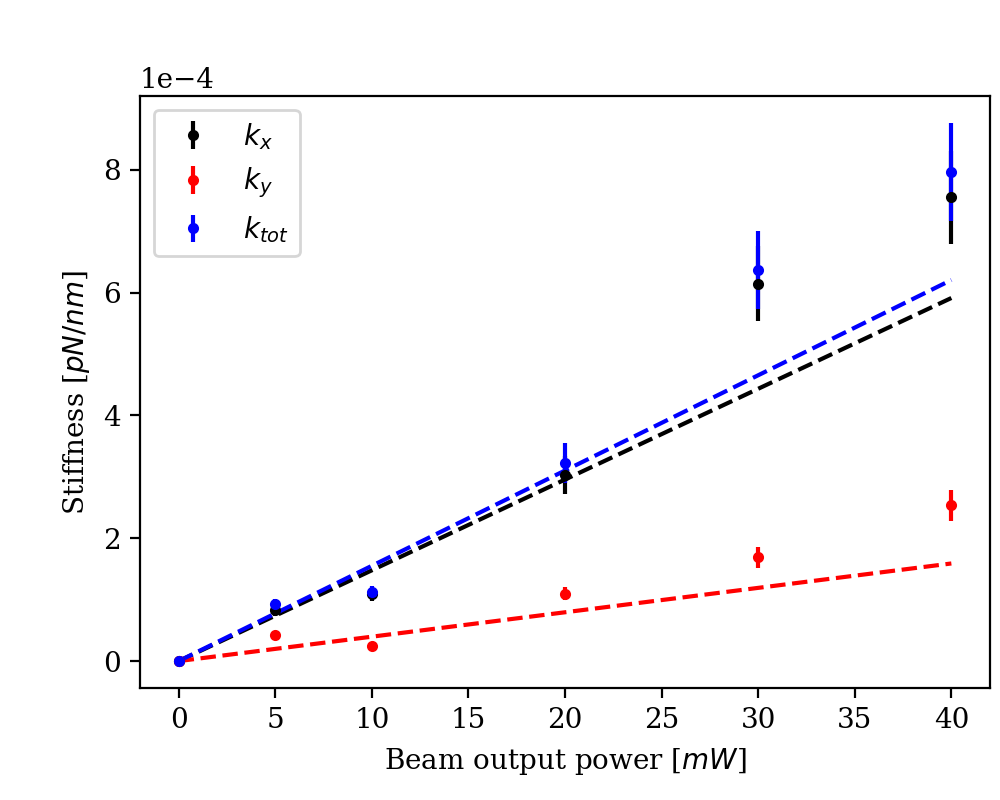
\includegraphics[width=\linewidth]{figures/trap.png}
            \caption{Results of the second dataset plotted and fitted.\\}
            \label{fig:trap-plot}
        \end{figure}
    \end{minipage}

\end{minipage}
\\

The data shown above in tables \ref{tab:first-results} and \ref{tab:second-results} are plotted in figures \ref{fig:bead-plot} and \ref{fig:trap-plot} re\-spectively. In the plots the in\-divi\-dual data points and their cor\-responding error flags are shown as well as the least squares fit of these data points for the $k_x$, $k_y$ and $k_{tot}$ values. The fit of the $k_{tot}$ values is plotted on a secondary axis.\\
For the least squares fit a relation of $k=a \cdot P$ was used since it is expected that for zero laser output power there would not be a restoring force acting on the particle. The resulting coefficients are shown below in table \ref{tab:fit-results}.\\

\vspace{-0.5cm}
\begin{table}[h!]
    \centering
    \begin{tabular}{|l|l|l|l|}
        \hline
        coefficient for & $a_x$ {[}$pN/(nm\cdot mW)${]} & $a_y$ {[}$pN/(nm \cdot mW)${]} & $a_{tot}$ {[}$pN/(nm \cdot mW)${]} \\ \hline
        dataset 1       & $1.382\cdot 10^{-6}$          & $1.280 \cdot 10^{-6}$          & $1.740 \cdot 10^{-4}$              \\ \hline
        dataset 2       & $1.478 \cdot 10^{-5}$         & $3.974 \cdot 10^{-6}$          & $1.551 \cdot 10^{-5}$              \\ \hline
    \end{tabular}
    \caption{fit results}
    \label{tab:fit-results}
\end{table}

\clearpage{}
\subsection{Python program results}